\documentclass[../document.tex]{subfiles}

\begin{document}

\section{User Installation Guide}

\subsection{System Setup}
Setting up the system involves setting up different individual system components. The main components are the central hub, the database, and the visualiser. Other components involve a network to connect the main components together, and a script to pull pull data from the central hub and push it to the visualiser. The steps in the process are the following:
\begin{enumerate}
\item Setting up a network

\item Setting up the central hub and the sensors

\item Setting up the database

\item Configuring the visualiser

\item Running the database
\item Running the visualiser
\item Running the script
\end{enumerate}

%TODO: Write about charging the sensors

\subsection{Setting up a network}
As the central hub can only run on a Raspberry Pi, a network is needed to connect it to the rest of the system. The Raspberry Pi is configured to get an IP address automatically through DHCP, so the network needs to have a DHCP server available. Normally the DHCP server is a router, but a laptop running Linux can also be setup to function as one. Regardless, it is recommended to setup your own dedicated network using either a router or a laptop, as it eases the next step considerably. Instructions for setting up a laptop running Linux as a DHCP server can be found here \url{http://www.cyberciti.biz/faq/howto-ubuntu-debian-squeeze-dhcp-server-setup-tutorial/}.
Setting up a DHCP server on windows involves a considerable amount of work, and is not recommended.

After the network is set up with a DHCP server, the different systems running the components will be assigned IP addresses automatically when they are connected.



\subsection{Setting up the central hub and the sensors}
The following accessories is needed to setup the central hub and the sensors:
\newcommand{\Imwidth}{0.40}
\begin{figure}[H]
	\centering
	\begin{subfigure}[h]{\Imwidth\textwidth}
		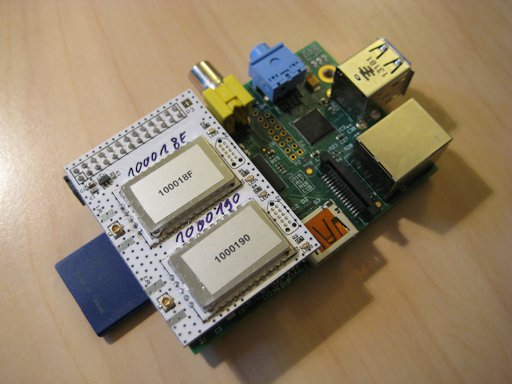
\includegraphics[width=\textwidth]{user_installation_guide/rpi.jpg}
		\caption{Raspberry Pi}	
	\end{subfigure}
	\quad
	\begin{subfigure}[h]{\Imwidth\textwidth}
		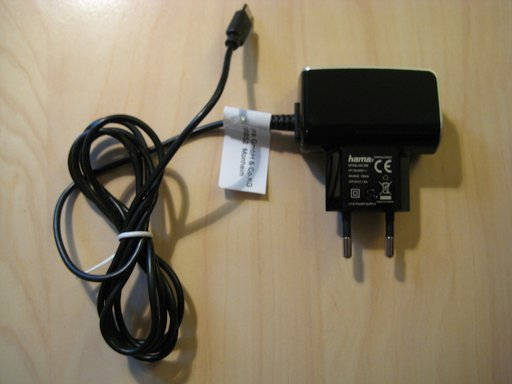
\includegraphics[width=\textwidth]{user_installation_guide/rpi-power-cord.jpg}
		\caption{Raspberry Pi power cord}	
	\end{subfigure}
	\quad
	\begin{subfigure}[h]{\Imwidth\textwidth}
		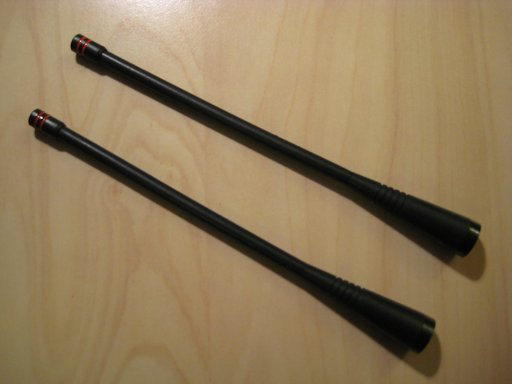
\includegraphics[width=\textwidth]{user_installation_guide/rpi-antenna.jpg}
		\caption{DASH7 antennas}	
	\end{subfigure}
	\quad
	\begin{subfigure}[h]{\Imwidth\textwidth}
		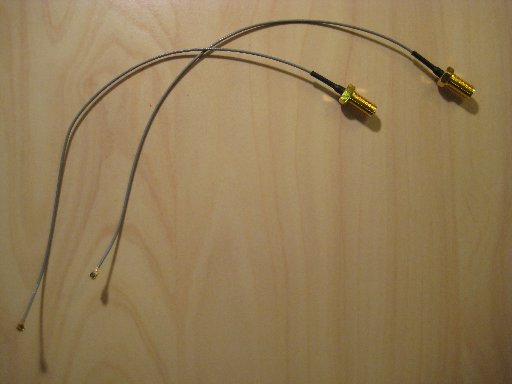
\includegraphics[width=\textwidth]{user_installation_guide/rpi-antenna-cable.jpg}
		\caption{Antenna signal cables}	
	\end{subfigure}
	\quad
	\begin{subfigure}[h]{\Imwidth\textwidth}
		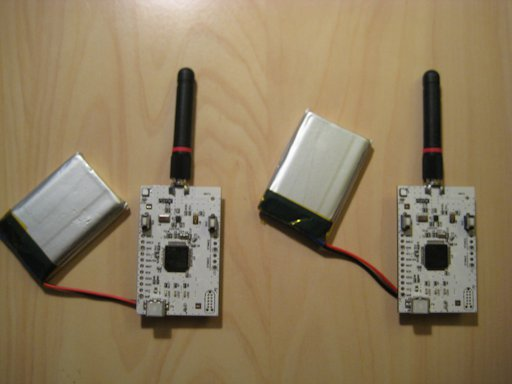
\includegraphics[width=\textwidth]{user_installation_guide/sensor.jpg}
		\caption{Sensors}	
	\end{subfigure}
	\quad
	\begin{subfigure}[h]{\Imwidth\textwidth}
		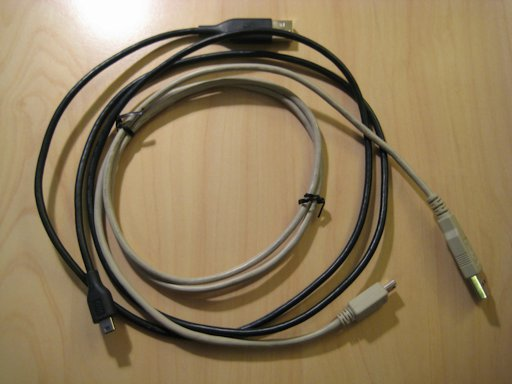
\includegraphics[width=\textwidth]{user_installation_guide/sensor-power-cord.jpg}
		\caption{Sensor power cords (optional)}	
	\end{subfigure}
	\quad
	\begin{subfigure}[h]{\Imwidth\textwidth}
		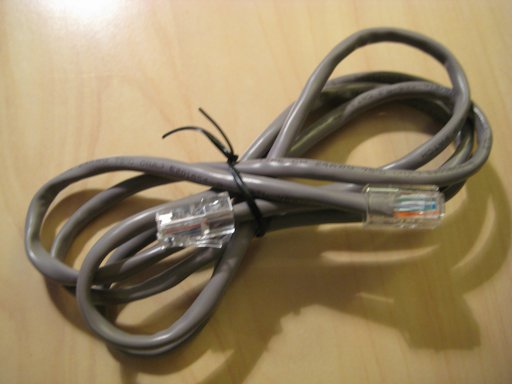
\includegraphics[width=\textwidth]{user_installation_guide/rpi-network-cable.jpg}
		\caption{Network cable}	
	\end{subfigure}
	\caption{Accessories needed to set up the central hub}
\end{figure}

To setup the central hub and the sensors, complete the steps outlined in the figures below:
\begin{figure}[H]
	\centering
	\begin{subfigure}[h]{0.48\textwidth}
		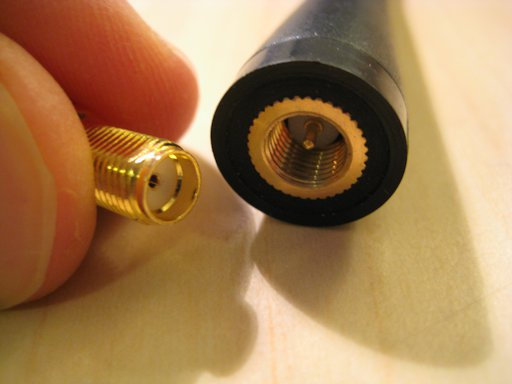
\includegraphics[width=\textwidth]{user_installation_guide/connect-antenna-cables.jpg}
	\end{subfigure}
	\quad
	\begin{subfigure}[h]{0.48\textwidth}
		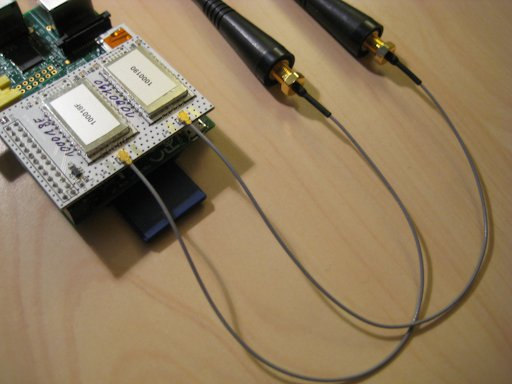
\includegraphics[width=\textwidth]{user_installation_guide/connect-rpi-antennas.jpg}
	\end{subfigure}
	\caption{Attach the antenna signal cables to the antennas, and connect the antenna signal cables to the Raspbery Pi}
\end{figure}

\begin{figure}[H]
	\centering
	\begin{subfigure}[h]{0.48\textwidth}
		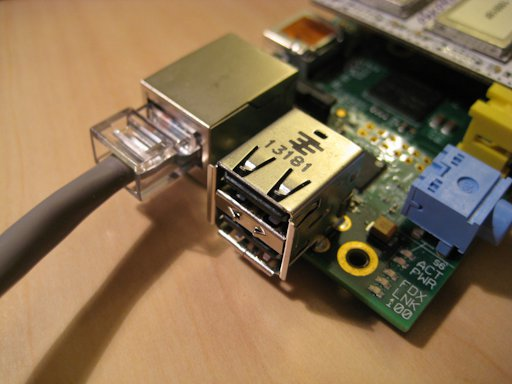
\includegraphics[width=\textwidth]{user_installation_guide/connect-rpi-network.jpg}
	\end{subfigure}
	\quad
	\begin{subfigure}[h]{0.48\textwidth}
		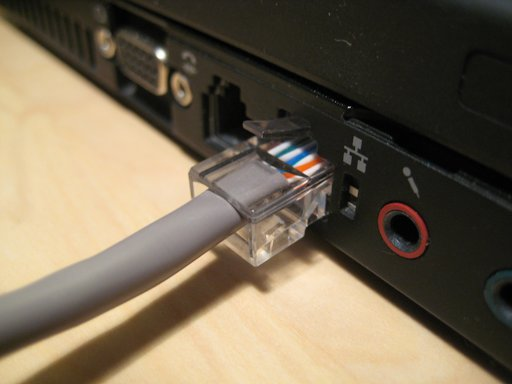
\includegraphics[width=\textwidth]{user_installation_guide/connect-rpi-network-2.jpg}
	\end{subfigure}
	\caption{Connect the Raspberry Pi to the router using the networking cable}
\end{figure}

\begin{figure}[H]
	\centering
	\begin{subfigure}[h]{0.48\textwidth}
		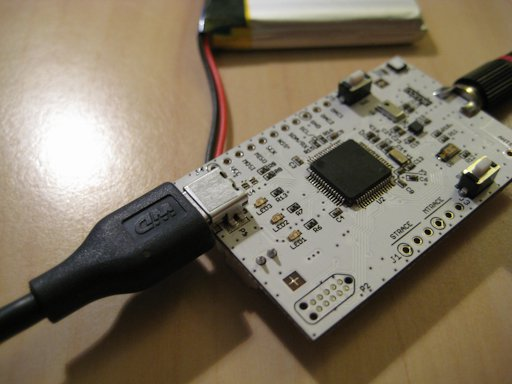
\includegraphics[width=\textwidth]{user_installation_guide/connect-sensor-power.jpg}
	\end{subfigure}
	\quad
	\begin{subfigure}[h]{0.48\textwidth}
		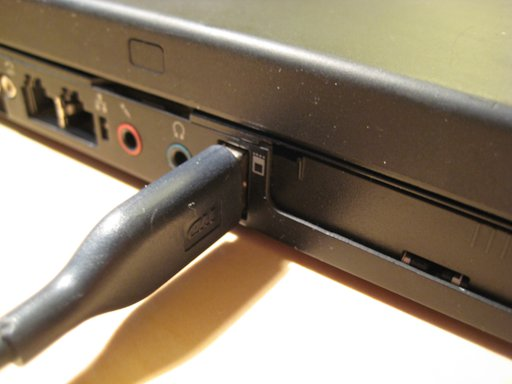
\includegraphics[width=\textwidth]{user_installation_guide/connect-sensor-power-2.jpg}
	\end{subfigure}
	\caption{Power the sensors by plugging one end of the sensor power cord into the sensor, and the other end into a powered USB port (optional)}
\end{figure}

\begin{figure}[H]
	\centering
	\begin{subfigure}[h]{0.48\textwidth}
		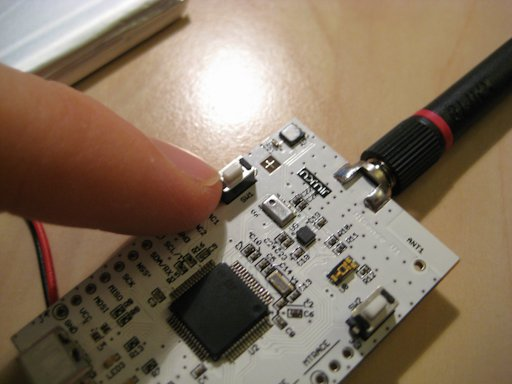
\includegraphics[width=\textwidth]{user_installation_guide/turn-on-sensors.jpg}
	\end{subfigure}
	\quad
	\begin{subfigure}[h]{0.48\textwidth}
		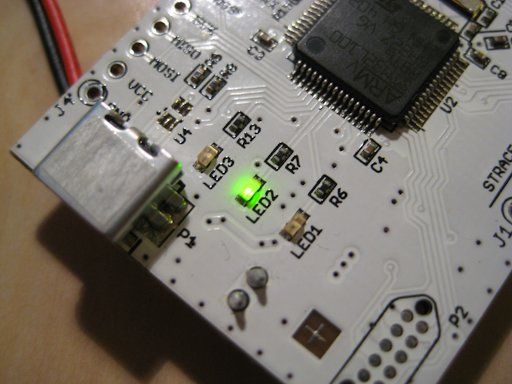
\includegraphics[width=\textwidth]{user_installation_guide/turn-on-sensors-2.jpg}
	\end{subfigure}
	\caption{Turn on the sensor by pressing the button to the left of the antenna. Keep the button depressed for at least one second, or until the green LED is lighted.}
\end{figure}

\begin{figure}[H]
	\centering
	\begin{subfigure}[h]{0.48\textwidth}
		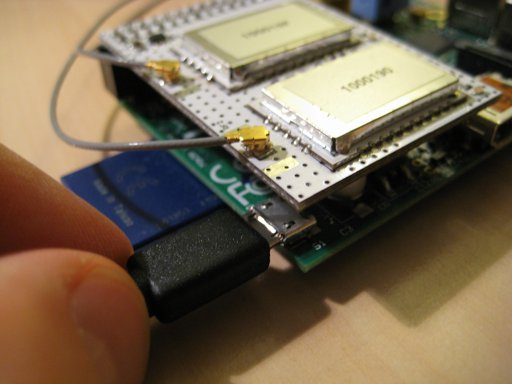
\includegraphics[width=\textwidth]{user_installation_guide/connect-rpi-power.jpg}
	\end{subfigure}
	\quad
	\begin{subfigure}[h]{0.48\textwidth}
		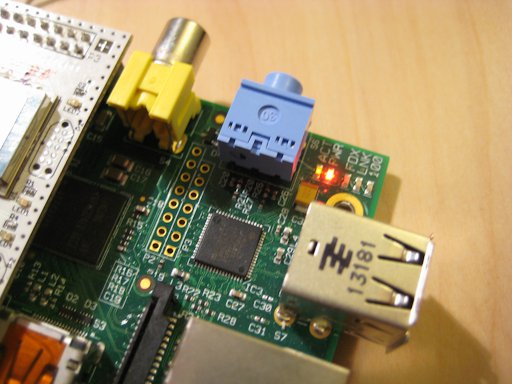
\includegraphics[width=\textwidth]{user_installation_guide/connect-rpi-power-2.jpg}
	\end{subfigure}
	\caption{Start the Raspberry Pi by plugging the power cord into it. The other end of the cord should be plugged into a power outlet. A red LED will light up indicating that the Raspberry is running.}
\end{figure}



\subsection{Acquiring IP Addresses}
In order to set up all the components of the system, it is necessary to know the IP addresses of the central hub and the database. As these addresses are assigned dynamically by the DHCP server, it is not possible to known them in advance. This section goes into detail about how to acquire the IP addresses.

For the central hub, the simplest way to discover the address is by trial and error. For this we need to know the address pool used by the DHCP server, so take note of this when setting up the network. The idea is to test subsequent addresses from this pool until the address of the central hub is found. The central hub runs a REST-based server, and the easiest way of testing an address is to type in the address in a browser. If the address is correct, this will open the configuration service of the central hub. It is likely that the central hub was leased an address in the lower end of the range, so it is a good idea to start there. For example, if the setup is performed on a local network, a typical lower end of the range address is 192.168.1.1.

If a laptop is used as a DHCP server, another option is also available. This involves viewing the log messages from the running DHCP server. The DHCP server will write the addresses it leases to the log, allowing you to read the address of the central hub.

It is also necessary to get the IP address of the database. Assuming the database is run on a computer with easy access to a terminal, this can be found using the command-line utility ipconfig in Windows, or ifconfig in OS X or Linux.
\begin{lstlisting}[caption=Example output of the ifconfig command in Linux]
$ ifconfig
wlan0     Link encap:Ethernet  HWaddr 00:18:de:01:f9:8c  
          inet addr:78.91.30.139  Bcast:78.91.31.255  Mask:255.255.252.0
          inet6 addr: fe80::218:deff:fe01:f98c/64 Scope:Link
          UP BROADCAST RUNNING MULTICAST  MTU:1500  Metric:1
          RX packets:94186 errors:0 dropped:0 overruns:0 frame:0
          TX packets:90496 errors:0 dropped:0 overruns:0 carrier:0
          collisions:0 txqueuelen:1000 
          RX bytes:32612781 (31.1 MiB)  TX bytes:40241945 (38.3 MiB)
\end{lstlisting}


\subsection{Starting the System Components}
At this point all devices are powered on, they are connected to the network, and the IP address of the central hub and the database has been acquired. The final step is to start the individual system components. These include the visualiser, the database, and a small script running on the Raspberry Pi. The central hub is started automatically by the Raspberry Pi on boot. It is important that the database already runs before the visualiser is started. Apart from that, the components can be started in any order. However, it is recommended to start them in the order specified below.

\subsubsection{Starting the Database}
The database receives sensor samples from the central hub, storing them in files. In order to start the database, open a terminal and navigate to the folder where the file the executable .jar file is located. Next, execute the .jar using the command
\begin{lstlisting}
$ java -jar IoT-service-0.9.1-SNAPSHOT-with-deps.jar
\end{lstlisting}
The database should now start printing log messages.



\subsubsection{Starting the pull script}
The script running on the Raspberry Pi along with the central hub is used pull sensor samples from the central hub and push them to the database. It is a Bash script that uses the command-line tool cURL to communicate with the central hub and the database. This script resides on the central hub under the path /home/root/push.sh. The recommended way to start the script, is to log on to the Raspberry Pi through ssh, using ‘root’ as both username and password. After logging in, the script is started with the command
\begin{lstlisting}
$ ./pull.sh <central hub ip> <database ip>
\end{lstlisting}
where the IP of the central hub and the database is specified as arguments.

The script can also be run on any computer connected to the network. Using a bash shell it can be pulled from the central hub with the command below.
\begin{lstlisting}[caption=Bash command to copy the central hub script. Note the period at the end.]
$ scp root@<central hub ip>:/home/root/pull.sh .
\end{lstlisting}
After copying the script, it is executed as mentioned above.

\subsubsection{Starting the Visualiser}
{\color{red} <Todo: Write about how the visualiser is started. Explicitly mention where you enter the IP address of the database>}


\subsection{System Configuration}
Some aspects of the different system components can be configured. In particular, the central hub can be configured in how it pulls data from the sensors. This configuration interface is accessed with a web browser, typing the IP address of the central hub into the address bar. Visiting the IP address should redirect the browser to a login screen. As before, use as login credentials ‘root’ as both username and password.
{\color{red} <Todo: Write about how to configure link budget in the visualiser>}



\end{document}
